\documentclass{article}
\usepackage{lucidabr,amsmath}
\usepackage{verbatim,fancyvrb}
\usepackage{color,mycode}
\usepackage{graphicx}
\usepackage[authoryear]{natbib}
\usepackage{smallhds,url}
\usepackage{hyperref}

\usepackage[letterpaper,body={6.3in,9.15in},top=.8in,left=1.1in]{geometry}
% \usepackage[a4paper,body={6.1in,9.7in},top=.8in,left=1.1in]{geometry}

\hypersetup{pdftitle={Almonreg 0.5},
            pdfauthor={Allin Cottrell},
            colorlinks=true,
            linkcolor=blue,
            urlcolor=red,
            citecolor=steel,
            bookmarks=true,
            bookmarksnumbered=true,
            plainpages=false
}

\begin{document}

\setlength{\parindent}{0pt}
\setlength{\parskip}{1ex}

\title{Almonreg 0.5}
\author{Allin Cottrell}
\maketitle

\section{The Almon lag model}

This package esimates an Almon lag or PDL (Polynomial Distributed Lag)
model.\footnote{The exposition of the Almon lag in this section is
  largely borrowed, with thanks, from D. S. G. Pollock---see
  \url{http://www.le.ac.uk/users/dsgp1/COURSES/TOPICS/Almonlag.pdf}.}
This model can be a useful way of reducing the number of parameters to
be estimated in the distributed lag model given by
%
\begin{equation}
\label{eq:dl}
y_t = \sum_{i=0}^p \beta_i x_{t-i} + \cdots + \varepsilon_t
\end{equation}
%
where the ellipsis indicates the possible presence of regressors
besides the lags of $x$.

In the Almon approach we assume that the $p+1$ coefficients
$\{\beta_i\}$ can be represented by the ordinates of a polynomial
$P(i)$ of degree $q$, with $q$ less than $p$. In that case we can
write
%
\begin{equation}
\label{eq:beta}
\beta_i = P(i) = \sum_{j=0}^q \gamma_j i^j \qquad i=0,\dots,p
\end{equation}

The equations (\ref{eq:beta}) may be written out explicitly as
%
\begin{equation*}
\left[
\begin{array}{c}
\beta_0 \\
\beta_1 \\
\beta_2 \\
\vdots \\
\beta_p \\
\end{array}
\right]
=
\left[
\begin{array}{ccccc}
1 & 1 & 1 & \cdots & 1 \\
1 & 2 & 4 & \cdots & 2^q \\
1 & 3 & 9 & \cdots & 3^q \\
\vdots & \vdots & \vdots & & \vdots \\
1 & p & p^2 & \cdots & p^q \\
\end{array}
\right]
\left[
\begin{array}{c}
\gamma_0 \\
\gamma_1 \\
\gamma_2 \\
\vdots \\
\gamma_q \\
\end{array}
\right]
\end{equation*}

Substituting from (\ref{eq:beta}) into (\ref{eq:dl}) we get
%
\begin{align}
y_t &= \sum_{i=0}^p \sum_{j=0}^q \gamma_j i^j x_{t-i} + \cdots +
\varepsilon_t \notag \\
 &= \sum_{j=0}^q \gamma_j z_{jt} + \cdots + \varepsilon_t
\end{align}
%
where $z_{jt} = \sum_{i=0}^p i^j x_{t-i}$. We can think of the $z_j$s
as ``artificial regressors,'' which can be constructed quite easily
given the time series for $x$. The procedure is then to run an OLS
regression of $y$ on the $z_j$s plus any other regular regressors.
With estimates of $\gamma_0,\dots,\gamma_q$ in hand, we can use
(\ref{eq:beta}) to compute estimates of the $\beta_i$s. Standard
errors for these estimates can be obtained via the delta method.

\section{Command-line usage}

The function available for command-line and scripting use is
named \texttt{almonreg}. It returns a bundle (to be described below)
and takes the following arguments:

\begin{center}
\begin{tabular}{llll}
  \textit{name} & \textit{type} & \textit{comment} & \textit{default value} \\[4pt]
  \textsl{y} & series & the dependent variable & --  \\ 
  \textsl{x} & series & for PDL treatment &  -- \\
  \textsl{p} & integer & the maximum lag & 4\\
  \textsl{q} & integer & the degree of the polynomial & 2\\
  \textsl{c} & boolean & include a constant? & 1 (yes)\\
  \textsl{X} & list & additional regressors & \texttt{null} \\
  \textsl{quiet} & boolean & quiet operation? & 0 (no)
\end{tabular}
\end{center}

We illustrate a call to this function by reference to the sample
script included in the package, which replicates the analysis of
\cite{almon65}. This script begins with
%
\begin{code}
include almonreg.gfn
open almon.gdt --frompkg=almonreg
\end{code}
%
The data file \texttt{almon.gdt} contains two quarterly time series
running from 1952Q1 to 1966Q4, namely \texttt{ce} (capital
expenditures) and \texttt{ca} (capital appropriations). These are
National Industrial Conference Board data, a variant of the data used
by Shirley Almon. The next two lines generate a list, \texttt{X},
containing dummy variables representing the first, second and third
quarters, to allow for seasonality.
%
\begin{code}
genr dummy
list X = dq1 dq2 dq3
\end{code}
%
We then select the lag and polynomial orders and invoke
\texttt{almonreg}, saving the result.
%
\begin{code}
scalar p = 5 # maximum lag length
scalar q = 2 # order of Almon polynomial
bundle B = almonreg(ce, ca, p, q, 1, X)
\end{code}
%
If we hadn't wanted to include seasonal dummies the function call
could have been abbreviated to
\begin{code}
bundle B = almonreg(ce, ca, p)
\end{code}
%
in which case the model would have used $q = 2$ and included a
constant, these being the defaults.

Partial output from the sample script is shown in
Listing~\ref{output}. The first block displays the results of the
initial OLS using the ``artificial regressors'' $z_j$, $j=0,1,2$.  The
second block shows the computed coefficients on current \texttt{ca}
and the 5 specified lags. The final portion exposes the contents of
the bundle returned by \texttt{almonreg}.

\begin{script}[htbp]
\begin{scodebit}
? bundle B = almonreg(ce, ca, p, q, 1, X)

OLS, using observations 1953:2-1966:4 (T = 55)
Dependent variable: y

             coefficient    std. error    t-ratio   p-value
  ---------------------------------------------------------
  const      210.011        73.2524        2.867    0.0061  ***
  dq1        -10.5515       61.0634       -0.1728   0.8635 
  dq2        -20.9887       59.9386       -0.3502   0.7277 
  dq3        -30.4337       59.9004       -0.5081   0.6137 
  z_0          0.0894672     0.0359914     2.486    0.0165  **
  z_1          0.0108136     0.0487294     0.2219   0.8253 
  z_2          0.00403575    0.00970653    0.4158   0.6794 

Mean dependent var   3185.691   S.D. dependent var   1159.091
Sum squared resid     1205186   S.E. of regression   158.4552
R-squared            0.983388   Adjusted R-squared   0.981311
F(6, 48)             473.5757   P-value(F)           6.14e-41
Log-likelihood      -352.8989   Akaike criterion     719.7979
Schwarz criterion    733.8492   Hannan-Quinn         725.2316
rho                  0.680651   Durbin-Watson        0.615720

Excluding the constant, p-value was highest for variable 3 (dq1)

Almon lag, polynomial order 2

             coefficient   std. error     z      p-value 
  -------------------------------------------------------
  ca          0.0894672    0.0359914     2.486   0.0129   **
  ca(-1)      0.104317     0.0109080     9.563   1.14e-21 ***
  ca(-2)      0.127237     0.0254693     4.996   5.86e-07 ***
  ca(-3)      0.158230     0.0253707     6.237   4.47e-10 ***
  ca(-4)      0.197294     0.0111510    17.69    4.75e-70 ***
  ca(-5)      0.244429     0.0370444     6.598   4.16e-11 ***

? print B
bundle B, created by almonreg:
  k = 4
  p = 5
  q = 2
  beta (matrix: 10 x 1)
  gamma (matrix: 7 x 1)
  se (matrix: 10 x 1)
  xname = "ca"
\end{scodebit}
  \caption{Partial output from sample script}
  \label{output}
\end{script}

\subsection{The returned bundle}

The bundle returned by \texttt{almonreg} contains the following items.
\begin{itemize}
\item The integers \texttt{p} and \texttt{q} passed in the user's
  input, plus an integer \texttt{k} giving the number of regressors
  besides the PDL term (including the constant if present).
\item Column vectors of length \texttt{k} + \texttt{p} + 1 named
  \texttt{beta} and \texttt{se} holding parameter estimates and their
  associated standard errors, respectively. These values refer, in
  order, to the constant (if present); the elements of \texttt{X} (if
  present); and the current and lagged values of the series subject to
  PDL treatment. They correspond to the first 4 lines of the OLS
  output shown in Listing~\ref{output} plus the 6 lines shown in the
  second output block.
\item A column vector \texttt{gamma} of length \texttt{k} + \texttt{q}
  + 1 holding the coefficients from the initial OLS regression of $y$
  on the $z_j$s and other terms.
\item Under the key \texttt{xname}, the name of the PDL series.

\end{itemize}

\section{GUI usage}

On installing the package you should be given the option of adding a
hook named \textsf{Almon lag} to gretl's \textsf{Model} menu, under
the \textsf{Univariate time series} sub-menu. This hook brings up a
dialog box in which you can select the various inputs described above
(Figure~\ref{fig:dialog}). Clicking \textsf{OK} in this dialog will
open a window displaying the results of estimation and allowing you to
save the results bundle and/or any of its contents.

\begin{figure}[htbp]
  \centering
  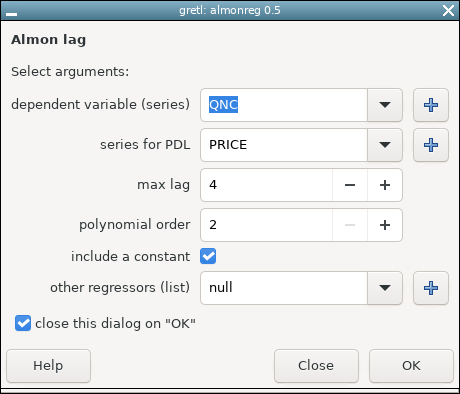
\includegraphics[scale=0.6]{almonreg.png}
  \caption{The almonreg dialog}
  \label{fig:dialog}
\end{figure}

\bibliographystyle{gretl}
\bibliography{gretl}

\end{document}
